\documentclass{article}

\makeatletter
\renewcommand*{\fps@figure}{!htb}
\renewcommand*{\fps@table}{!htb}
\makeatother

\usepackage[utf8]{inputenc}
\usepackage[hidelinks]{hyperref}
\usepackage{amsmath, bm}
\usepackage[capitalise, nameinlink]{cleveref}
\usepackage{amssymb}
\usepackage{graphicx}
\usepackage{float}
\usepackage{booktabs}
\usepackage[parfill]{parskip}
\usepackage{comment}
\usepackage{subcaption}

\usepackage[sorting=none]{biblatex}
\addbibresource{report_3.bib}

\usepackage{titling}
\setlength{\droptitle}{-3cm}

\title{COMP6247 Lab 3: Kalman and Particle Filters; Online PCA}
\author{Wei Chien Teoh (Eugene)\\\bigskip \href{mailto:wct1c16@soton.ac.uk}{wct1c16@soton.ac.uk}}
\date{16 April 2021}

\begin{document}

\maketitle

\section{Introduction}

This report presents the findings and results for Lab 3 of COMP6247 \cite{lab3}. The code implementation is stored in a Github repository \cite{github}.

\section{Task 1}

Task 1 presents my implementation of the Sequential Importance Sampling (SIS) and Sequential Importance Resampling (SIR). The results of SIS and SIR will be compared to the Kalman Filter (KF) implementation \cite{lab2ans} for the state estimation of the time-varying autoregressive time series problem stated in Lab 2 \cite{lab2}.

A second-order time-varying autoregressive time series identical to \cite{lab2} is generated with a time index, $T$ of 200.

Initially, the Sequential Importance Sampling (SIS) algorithm described in \cite{particle_filters} was implemented. However, due to the recursive multiplication of weights, almost all particle weights becomes infinitesimally small except for one. This behaviour is shown in \cref{fig:sis-particle-weights}, where initially the size of the weights are equal. After several iterations, the weights are mostly focused on only one particle. This phenomenon is known as weight degeneracy. This signifies that the posterior distribution is majorly dependent on only one particle.

To solve weight degeneracy, an extra resampling step \cite{particle_filters} is added to the original SIS algorithm, which is then known as Sequential Importance Resampling (SIR). For every iteration, the weights are resampled to have equal sizes, shown in \cref{fig:sir-particle-weights}. \cref{fig:ess} shows the Effective Sample Size (ESS) before and after introducing the resampling step. With resampling introduced, larger number of particles are effectively accounted to the estimation of the posterior PDF.

% TODO: mention that resampling doesnt have to happen at every iteration but when ESS is at a value below a threshold.

\cref{fig:results-1} shows the estimation of parameters $a_0$ and $a_1$ of the second-order time varying auto-regressive time series using a Kalman Filter implemented in \cite{lab2ans}, SIS and SIR. It is shown that all three algorithms did not provide ``smooth'' estimations. This is potentially due to the original process model described in \cite{lab2} being a random walk model instead of being non-linear. The Mean Squared Error (MSE) calculated for the three algorithm implies that the performance is in the order: SIS, KF, SIR.

\begin{comment}
- N = 500; Ns = 100;

- weight degeneracy
- weights are < 1, therefore it will be infinitesimally small after it is multiplied by many times during weight update.
- as large time index goes by, weight degeneracy occurs, ess converges to 1
- the posterior pdf is only dependent on one particle, which is bad
- can be solved by resampling
\end{comment}

\begin{figure}
    \begin{subfigure}{.5\textwidth}
        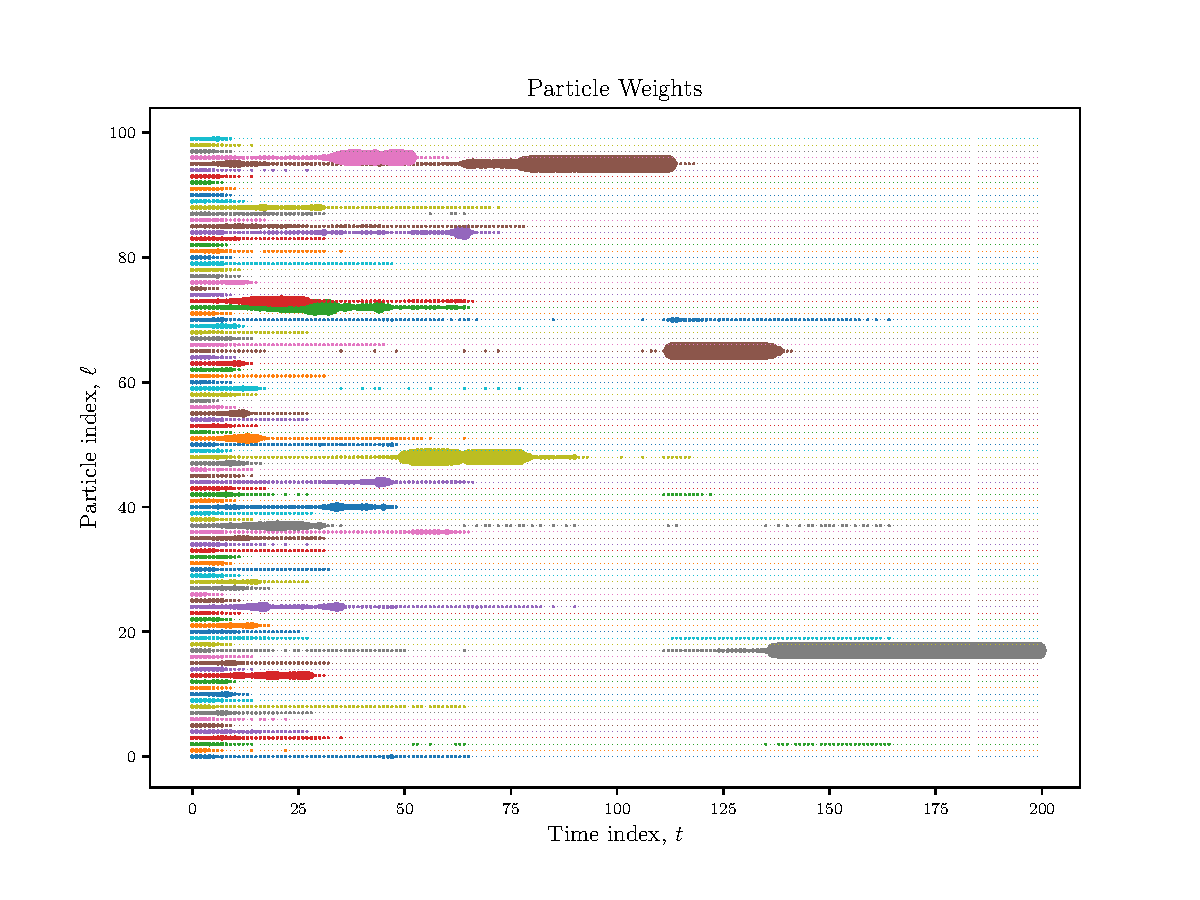
\includegraphics[width=1.15\textwidth]{Figures/particle_weights_sis.pdf}
        \caption{SIS}
        \label{fig:sis-particle-weights}
    \end{subfigure}
    \begin{subfigure}{.5\textwidth}
        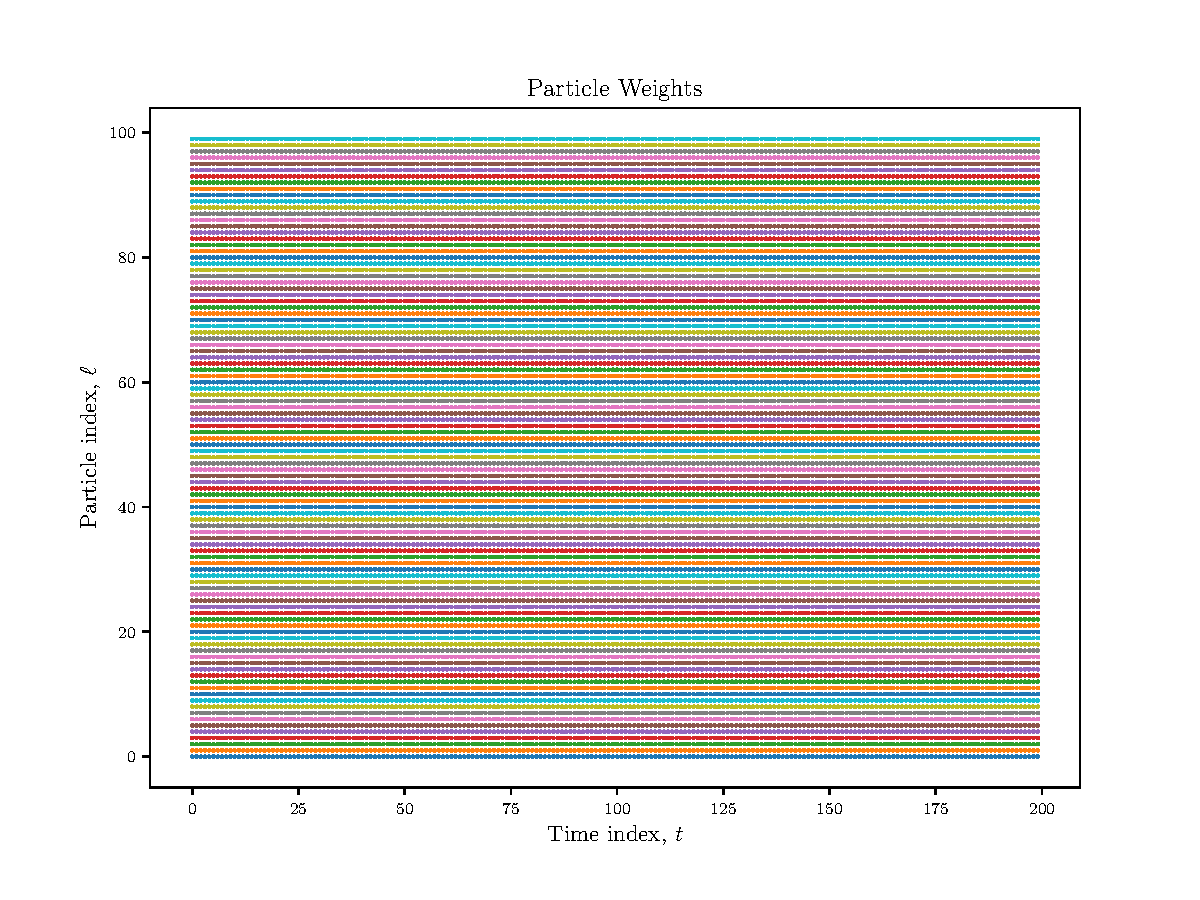
\includegraphics[width=1.15\textwidth]{Figures/particle_weights_sir.pdf}
        \caption{SIR}
        \label{fig:sir-particle-weights}
    \end{subfigure}
    \caption{Plot of particle weight size at each time step. The diameter of markers scales with the size of particle weights.}
    \label{fig:particle-weights}
\end{figure}

\begin{figure}
    \centering
    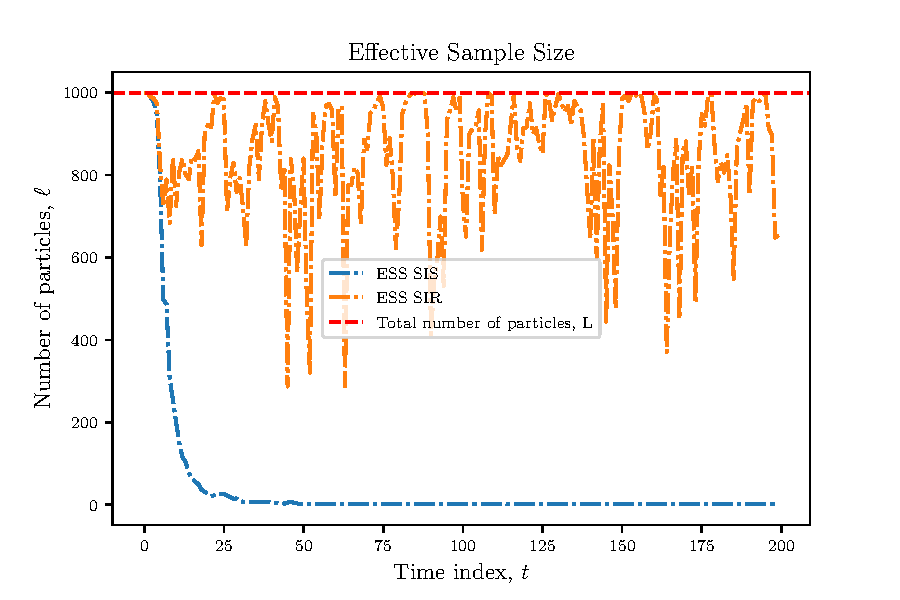
\includegraphics[width=.7\textwidth]{Figures/ess.pdf}
    \caption{Effective sample size of SIS and SIR algorithm.}
    \label{fig:ess}
\end{figure}

\begin{figure}
    \begin{subfigure}{.5\textwidth}
        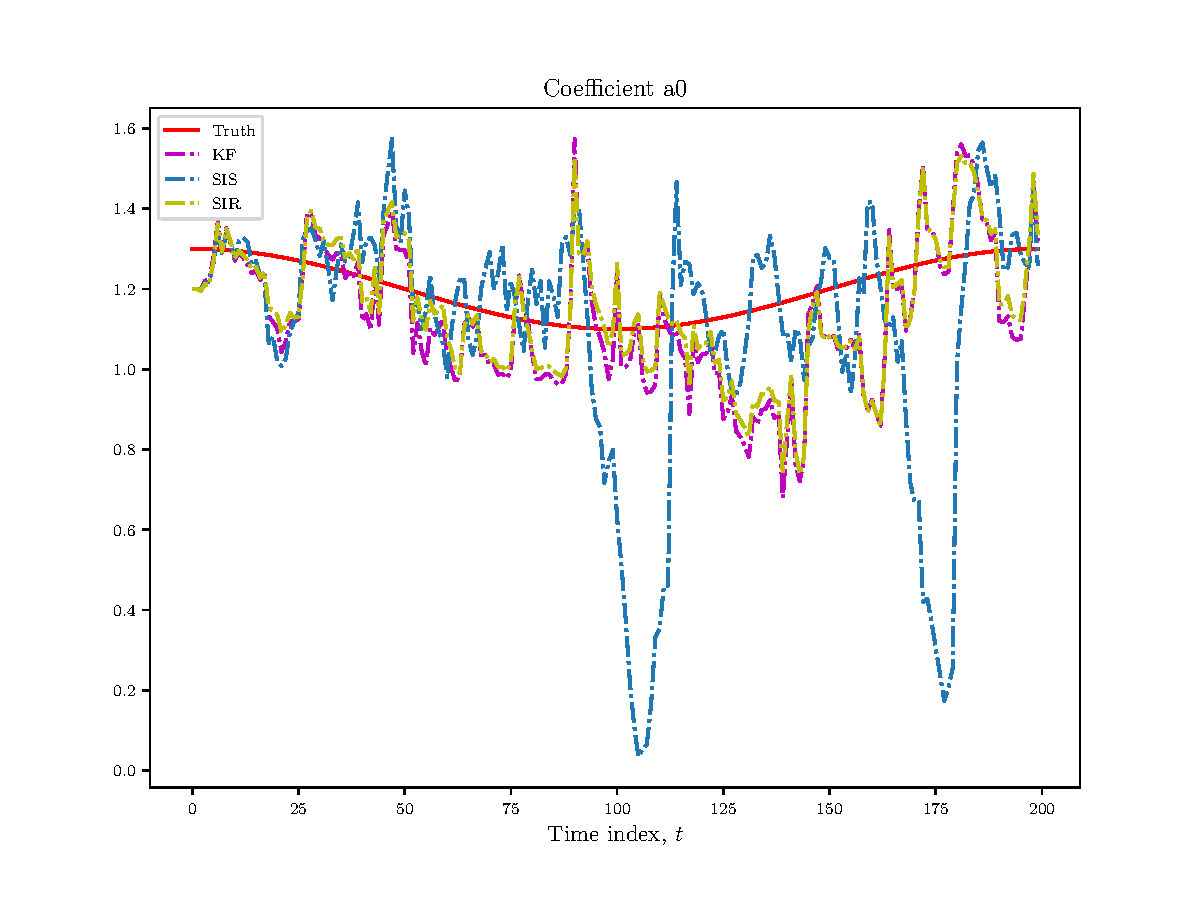
\includegraphics[width=1.15\textwidth]{Figures/coefficient_a0.pdf}
    \end{subfigure}
    \begin{subfigure}{.5\textwidth}
        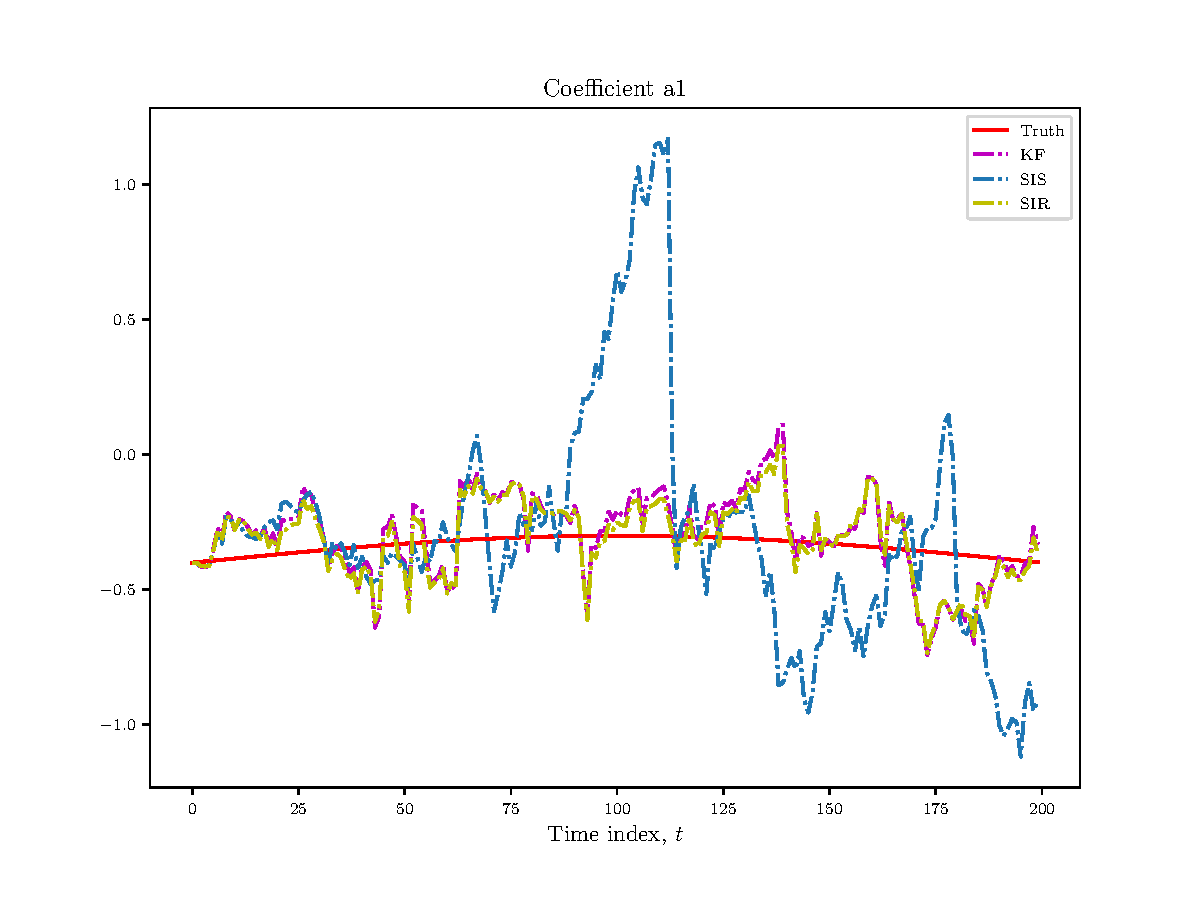
\includegraphics[width=1.15\textwidth]{Figures/coefficient_a1.pdf}
    \end{subfigure}

    \centering
    \begin{subfigure}{.7\textwidth}
        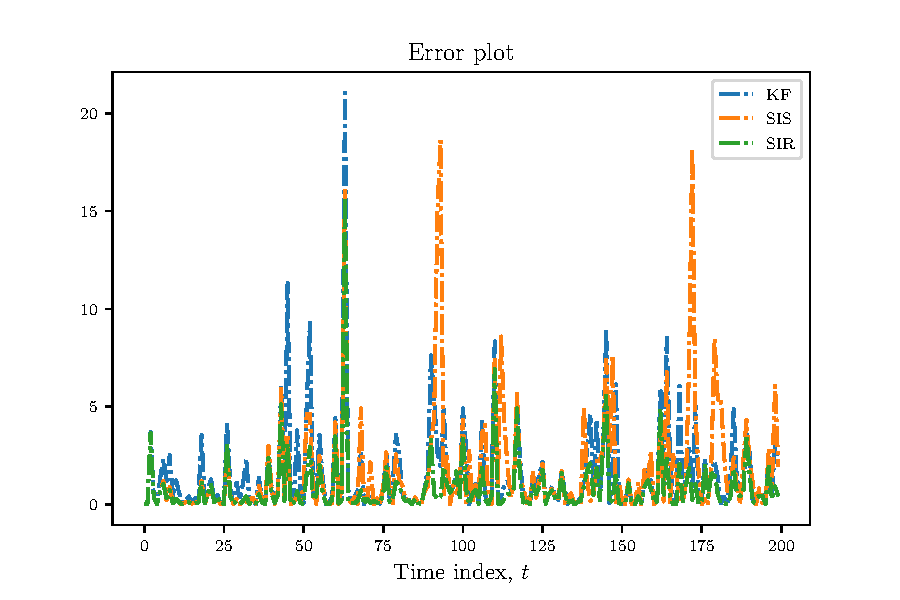
\includegraphics[width=\textwidth]{Figures/error.pdf}
    \end{subfigure}
    \caption{Plots of unknown parameters $a_0$ and $a_1$ estimated using KF, SIS and SIR, along with its squared errors. Mean Squared Error: (KF) 1.5617 (SIS) 1.6764 (SIR) 0.8354}
    \label{fig:results-1}
\end{figure}


\section{Task 2}

\section{Task 3}

\printbibliography

\end{document}